
\chapter*{Schr{\"o}dinger\rq s Equation}
\addcontentsline{toc}{chapter}{Schr{\"o}dinger\rq s Equation} 
\section*{Derivations}
\addcontentsline{toc}{section}{Derivations} 

	\marginpar{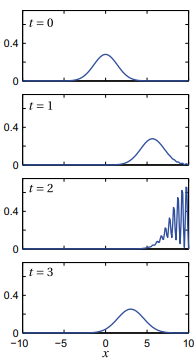
\includegraphics[width=\marginparwidth]{fig81}\captionof{figure}{The probability density $|\psi(x)|^{2}$ of a particle in a box that initially moves to the right and then interferes with itself as it reflects from an infinite potential (Problem 8.2(a)).}\label{fig:38}}
Here is the time-dependent Schr{\"o}dinger equation which governs the way a quantum wave function changes with time in a one-dimensional potential well $V(x)$:
\begin{equation}\label{eq:81}
i \bar{h} \frac{\partial \psi}{\partial t}=-\frac{\bar{h}^{2}}{2 m} \frac{\partial^{2} \psi}{\partial x^{2}}+V(x) \psi
\end{equation}
Note that except for the presence of the imaginary unit i, this is very much like
the diffusion equation. In fact, a good way to solve it is with the Crank-Nicolson
algorithm. Not only is this algorithm stable for Schr{\"o}dinger\rq s equation, but it has
another important property: it conserves probability. This is very important. If
the algorithm you use does not have this property, then as $\psi$ for a single particle
is advanced in time you have (after a while) 3/4 of a particle, then 1/2, etc. \\
\marginpar{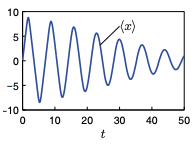
\includegraphics[width=\marginparwidth]{fig82}\captionof{figure}{The expectation position $\langle x\rangle$ for the particle in Fig. 8.1 as time progresses and the packet spreads out (Problem 8.2(c)).}\label{fig:39}}
The Schr{\"o}dinger equation usually describes the behavior of very tiny things
on very short timescales, so SI quantities like kilograms, meters, and Joules are
essentially infinite in quantum mechanics. Instead, we\rq ll use a system of units
called atomic units. In this system, lengths are measured in units of $a_0$ (the Bohr
radius, $a_0 = 5.29×10^{−11}$), masses are measured in units of the electron mass me ,
energies are measured in units of $E_0$ ($E_0 = \alpha^2mc^2 \approx 27 eV$), and time is measured
in units of $t_0 (t_0 = 24.2 attoseconds)$. These base units are chosen so that the
constants $\bar{h}$ and $m$ both have the numerical value of 1 (e.g. $m = 1m_e$ for an electron).
\begin{problem}\label{P8.1}
Use paper and pencil to derive a Crank-Nicolson algorithm to solve the
Schr{\"o}dinger equation. It will probably be helpful to use the material in
Lab 7 as a guide (beginning with Eq. \eqref{eq:715}). Make sure the $V(x)\psi$ term\end{problem}
enters the algorithm correctly
\section*{Particle in a box}
\addcontentsline{toc}{section}{Particle in a box} 
Let\rq s use this algorithm for solving Schr{\"o}dinger\rq s equation to study the evolution
of a particle in a box with
\begin{equation}\label{eq:82}
V(x)= \begin{cases}0 & \text { if }-L<x<L \\ +\infty & \text { otherwise }\end{cases}
\end{equation}
The infinite potential at the box edges is imposed by forcing the wave function to
be zero at these points:
\begin{equation}\label{eq:83}
\psi(-L)=0 \quad ; \quad \psi(L)=0
\end{equation}

\begin{problem}\label{P8.2}
\marginpar{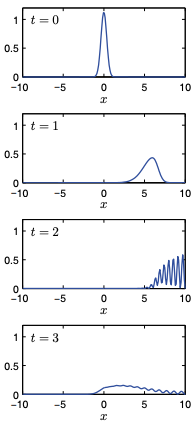
\includegraphics[width=\marginparwidth]{fig83}\captionof{figure}{The probability density $|\psi(x)|^{2}$ of a particle that is initially more localized quickly spreads (Problem 8.2(d)).}\label{fig:40}}
Modify one of your programs from Lab 7 to implement the Crank-Nicolson algorithm derived above for the case of a particle in a box with $L = 10$. Note we are doing quantum mechanics and the imaginary parts matter now. When assigning complex variables in NumPy, you use the engineering complex number $j$, like this:
\begin{lstlisting}
a = 1.0 + 0.5j
\end{lstlisting}
When you allocate your arrays, you\rq ll need to specify up-front that they will
hold complex values, like this:
\begin{lstlisting}
A = np.zeros((N,N),dtype=np.complex_)
B = np.zeros_like(A,dtype=np.complex_)
\end{lstlisting}
\marginpar{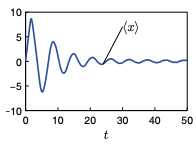
\includegraphics[width=\marginparwidth]{fig84}\captionof{figure}{The expectation position of the particle in Fig. 8.3 as time progresses.}\label{fig:41}}
\begin{enumerate}[label=(\alph*)]
	\item  Write a script to solve the time-dependent Schr{\"o}dinger equation using
Crank-Nicolson. We find that a cell-edge grid is easiest, but you can
also do cell-center with ghost points if you like. Start with a localized
wave packet of width $\sigma$ and momentum $p$:

\begin{equation}\label{eq:84}
\psi(x, 0)=\frac{1}{\sqrt{\sigma \sqrt{\pi}}} e^{i p x / \bar{h}} e^{-x^{2} /\left(2 \sigma^{2}\right)}
\end{equation}
with $p = 2\pi$ and $\sigma = 2$. (Remember that $ \bar{h}$ in \eqref{eq:84} has the numerical
value of 1 in our units.) This initial condition does not exactly satisfy
the boundary conditions, but it is very close. Check to see how far
off it is at the boundary, and decide how the sizes of $L$ and σ must
compare in to use this initial condition.
Run the script with $N = 200$ and watch the particle (wave packet)
bounce back and forth in the well. Plot the real part of $\psi$ as an animation to visualize the spatial oscillation of the wave packet, then
plot an animation of $\psi * \psi$  so that you can visualize the probability
distribution of the particle. Try switching the sign of $p$ and see what
happens.
\item Verify by doing a numerical integral that $\psi(x,0)$ in the formula given
above is properly normalized. Then run the script and check that
the wave packet stays properly normalized, even though the wave
function is bouncing and spreading within the well. If you are on a
cell-edge grid you should do the integrals with NumPy\rq s trapz rather
than sum.
\item Run the script and verify by numerical integration that the expectation
value of the particle position
\begin{equation}\label{eq:85}
\langle x\rangle=\int_{-L}^{L} \psi^{*}(x, t) x \psi(x, t) d x
\end{equation}
is correct for a bouncing particle. Plot $<x>(t)$ to see the bouncing
behavior. Run long enough that the wave packet spreading modifies
the bouncing to something more like a harmonic oscillator. (Note:
you will only see bouncing-particle behavior until the wave packet
spreads enough to start filling the entire well.)
\item You may be annoyed that the particle spreads out so much in time.
Try to fix this problem by narrowing the wave packet (decrease the
value of $\sigma$ ) so the particle is more localized. Run the script and explain
what you see in terms of quantum mechanics.


\end{enumerate}\end{problem}
\section*{Tunneling}
\addcontentsline{toc}{section}{Tunneling} 
	\marginpar{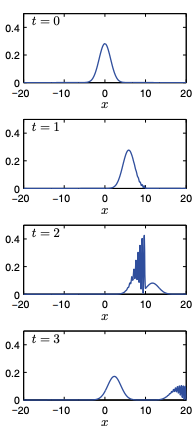
\includegraphics[width=\marginparwidth]{fig85}\captionof{figure}{he probability distribution $|\psi(x)|^{2}$ for a particle incident on a narrow potential barrier located just before $x=10$ with $\left.V_{0}\right\rangle\langle E\rangle$. Part of the wave tunnels through the barrier and part interferes with itself as it is reflected.}\label{fig:42}}
Now we will allow the pulse to collide with a with a non-infinite potential barrier
of height $V_0$ and width $\delta x = 0.02L$, and study what happens. Classically, the
answer is simple: if the particle has a kinetic energy less than $V_0$ it will be unable
to get over the barrier, but if its kinetic energy is greater than $V_0$ it will slow down
as it passes over the barrier, then resume its normal speed in the region beyond
the barrier. (Think of a ball rolling over a bump on a frictionless track.) Can
the particle get past a barrier that is higher than its kinetic energy in quantum
mechanics? The answer is yes, and this effect is called tunneling. \\ 
To see how the classical picture is modified in quantum mechanics we must
first compute the energy of our pulse so we can compare it to the height of the
barrier. The quantum mechanical formula for the expectation value of the energy
is
\begin{equation}\label{eq:86}
\langle E\rangle=\int_{-\infty}^{\infty} \psi^{*} H \psi d x
\end{equation}
where $\psi^∗$ is the complex conjugate of $\psi$ and where
\begin{equation}\label{eq:87}
H \psi=-\frac{\bar{h}^{2}}{2 m} \frac{\partial^{2} \psi}{\partial x^{2}}+V(x) \psi(x)
\end{equation}
In our case the initial wave function $\psi(x,0)$ given by Eq. \eqref{eq:84} is essentially zero at
the location of the potential barrier, so we may take $V(x) = 0$ in the integral when
we compute the initial energy. Performing the integral, we find
\begin{equation}\label{eq:88}
\langle E\rangle=\frac{p^{2}}{2 m}+\frac{\bar{h}^{2}}{4 m \sigma^{2}}
\end{equation}
Since this is a conservative system, the energy should remain constant throughout
the propagation.
\begin{problem}\label{P8.3}
\begin{enumerate}[label=(\alph*)]
	\item Modify your script from Problem 8.2 so that it uses a computing region hat goes from $-2L$ to $3L$ and a potential
\begin{equation}\label{eq:89}
V(x)= \begin{cases}0 & \text { if }-2 L<x<0.98 L \\ V_{0} & \text { if } 0.98 L \leq x \leq L \\ 0 & \text { if } L<x<3 L \\ +\infty & \text { otherwise }\end{cases}
\end{equation}
so that we have a square potential hill $V(x) = V_0$ between $x = 0.98L$ and $x = L$ and $V = 0$ everywhere else in the well.
Note: Since $V(x)$ was just zero in the last problem, this is the first time
to check if your $V(x)$ terms in Crank-Nicolson are right. If you see
strange behavior, you might want to look at these terms in your code.
\item Run your script several times, varying the height $V_0$ from less than your pulse energy to more than your pulse energy. Overlay a plot
of $V(x)/V_0$ on your plot of $ \vert \psi\vert^2$ and look at the behavior of $\psi$ in the barrier region. You should do several experiments with your code. (1) Try making
the barrier height both higher than your initial energy and lower than
your initial energy. Explain to your TA how the quantum behavior
differs from classical behavior. You should find that even when the
barrier is low enough that a classical particle could get over it, some
particles still come back. (2) Experiment with the width of your barrier
and see what its effect is on how many particles tunnel through. As
part of this experiment, figure out a way to calculate what fraction of
the particles make it through the barrier.

\end{enumerate}
\end{problem}